\chapter{Large sets and rapidly growing functions}\label{chap:alpha-large}

\begin{remark}
Some notations (mainly names of fast-growing functions) of our development may differ slightly from the literature. Although this fact does not affect our proofs, we are preparing a future version where the names $F_\alpha$, $f_\alpha$, $H_\alpha$, etc., are fully consistent with the cited articles.

\end{remark}
%\section{Introduction}

In this chapter, we try to feel how long a standard battle can be.
To be precise, for any ordinal $\alpha<\epsilon_0$ and any positive integer $k$,
we give a minoration of the number of steps of a standard battle which
starts with the hydra $\iota(\alpha)$ and the replication factor $k$.

We express this number in terms of the Hardy hierarchy of fast-growing 
functions~\cite{BW85, Wainer1970, KS81, Promel2013}.
 From the \coq{} user's point of view, such  functions are  very 
attractive:  they are defined as functions  in \gallina{}, and we can apply them \emph{in theory}, but they are so complex that you will never be able to look at the result of the computation.
 Thus, our knowledge on these functions must rely on \emph{proofs}, not tests. In our development, we use often the rewriting rules generated by \coq's \texttt{Equations} plug-in.


\section{Definitions}

%\subsection{Definition}

\begin{definition}
Let $0<\alpha<\epsilon_0$ be any ordinal, and $s=\langle s_1, s_2, \dots, s_N\rangle$ a finite sequence of strictly positive natural numbers. 

We say that $s$ is \emph{$\alpha$-large} if the sequence $\langle \alpha_0=\alpha,\dots,\alpha_{i+1}=\canonseq{\alpha_i}{i+1},\dots \rangle$ leads to $0$. 
We say also that $s$ is \emph{minimally $\alpha$-large} (in short:
\emph{$\alpha$-mlarge}) if $s$ is $\alpha$-large 
 and every strict prefix of $s$ leads to a non-zero ordinal (\emph{cf} Sect.~\vref{sect:path-to-def}).

\index{maths}{Ordinal numbers!Large sets}
\index{maths}{Ordinal numbers!Minimal large sets}

\end{definition}



\begin{remark}
  Ketonen and Solovay~\cite{KS81} consider  large finite \emph{sets} of natural numbers,  but they are mainly used as sequences. Thus, we chose to represent them explicitely as (sorted) lists. 
\end{remark}


The following function ``gnaws'' an ordinal $\alpha$, following a sequence of indices (ignoring the $0$s).

\vspace{4pt}

\noindent
\emph{From Module~\href{../theories/html/hydras.Epsilon0.Paths.html\#gnaw}{Epsilon0.Paths}}

\input{movies/snippets/Paths/gnawDef}


\noindent
\emph{From Module~\href{../theories/html/hydras.Epsilon0.Large_SetsPaths.html\#gnaw}{Epsilon0.Large\_Sets}}


\input{movies/snippets/Large_Sets/largeDef}



Minimal large sequences can be directly defined in terms of the
predicate \texttt{path\_to} (\vref{sect:path-to-def}) which already prohibits paths containing non-final \texttt{zero}s.

\vspace{4pt}

\noindent
\emph{From Module~ \href{../theories/html/hydras.Epsilon0.Large_Sets.html\#mlarge}{Epsilon0.Large\_Sets}}


\index{hydras}{Library Epsilon0!Predicates!mlarge@mlarge (minimal large sequences)}

\input{movies/snippets/Large_Sets/mlargeDef}


Let us consider two integers $k$ and $l$, such that $0<k<l$. In order to check whether the interval $[k,l]$ is minimally large for $\alpha$, it is enough to
follow from $\alpha$ the path associated with the interval $[k,l)$ and verify that the last ordinal we obtain is equal to $1$.
 
\subsection{Examples}

For instance the interval $[6,70]$ leads $\omega^2$ to $\omega\times 2 + 56$. Thus this interval is not $\omega^2$-large.



\noindent
\emph{From Module~ \href{../theories/html/hydras.Epsilon0.Large_Sets_Examples.html\#mlarge}{Epsilon0.Large\_Sets\_Examples}}

\input{movies/snippets/Large_Sets_Examples/gnawEx1}

The interval $[6,700]$ is $\omega^2$-large, but not
$\omega^2$-mlarge, since $[6,699]$ is also $\omega^2$-large.


\input{movies/snippets/Large_Sets_Examples/gnawEx2}

The following lemma relates minimal largeness with the
function 
\texttt{gnaw}. 

\input{movies/snippets/Large_Sets/mlargeIff}

\vspace{4pt}
 \noindent
\emph{From Module~\href{../theories/html/hydras.Epsilon0.Large_Sets_Examples.html}{Epsilon0.Large\_Sets\_Examples}}

\input{movies/snippets/Large_Sets_Examples/Ex1Lemma}

\section{Length of minimal large sequences}
\label{sect:lalpha-section}

Now, let us consider some natural number $k>0$ and an ordinal $0<\alpha<\epsilon_0$.  We would like to compute
a number $l$ such that the interval $[k,l]$ is $\alpha$-mlarge. So, 
the standard battle starting with $\iota(\alpha)$ and the replication factor $k$ will end after $(l-k+1)$ steps.



First, we notice that this  number $l$ exists, since the segment $[0,\epsilon_0)$ is well-founded and $\canonseq{\alpha}{i}<\alpha$ for any $i$ and $\alpha>0$.
Moreover, it is unique:

\vspace{4pt}
\noindent
\emph{From Module~\href{../theories/html/hydras.Epsilon0.Large_Sets.html}{Epsilon0.Large\_Sets}}

\input{movies/snippets/Large_Sets/mlargeUnicity}


Thus, we would like to define a function, parameterized by $\alpha$ which associates to any  strictly positive integer $k$ the number $l$ such that
the interval $[k,l]$ is $\alpha$-mlarge. It would be fine to write in \gallina{} a definition like this:

\begin{Coqbad}
Function L_ (alpha: E0) (i:nat) :  nat := ...
\end{Coqbad}

But we do not know how to fill the dots yet \dots{}   In the next section, we will 
use \coq{} to reason  about the \emph{specification} of \texttt{L},
prove properties of any function which satisfies this specification.
In Sect.~\ref{sect:L-equations}, we use the \texttt{coq-equations} plug-in
to define  \texttt{L\_}, then prove its correctness w.r.t. its specification.


\subsection{Formal specification}


Let $0<\alpha<\epsilon_0$ be an ordinal term. We consider any  function which  maps  any strictly positive integer $k$ to the number $l$, where 
the interval $[k,l)$ is $\alpha$-mlarge.

\begin{remark}
In~\cite{KS81} Ketonen and Solovay consider the least natural number $l$ where the interval $[k,l]$ ($l$ included) is $\alpha$-large, and call $H_\alpha$ the function which maps $k$ to $l$. We chose to consider intervals $[l,k)$ instead of $[l,k]$
in order to simplify  some statements and proofs in composition lemmas associated with the ordinals of the form $\alpha\times i$ and 
$\omega^\alpha\times i + \beta$.
Clearly, both approaches are related through the equality
$L_\alpha(k)=H_\alpha(k)+1$, for any non-null $\alpha$ and $k$.
\end{remark}




Our specification of the function \texttt{L} is as follows:

\emph{From Module~\href{../theories/html/hydras.Epsilon0.Large_Sets.html}{Epsilon0.Large\_Sets}}

\input{movies/snippets/Large_Sets/LSpecDef}


\begin{todo}
 Check if the functions $L_\alpha$ are the same as
\cite{KS81}' functions $f_\alpha$ (p. 297).
\end{todo}


Note that, for $\alpha\not=0$, the value of $f(0)$ is not specified.
Nevertheless, the restriction of $f$ to the set of strictly positive integers is unique (up to extensionality).

\input{movies/snippets/Large_Sets/LSpecUnicity}


\subsection{Abstract properties}



Let us now prove properties of any function $f$ (if any) which satisfies 
\texttt{L\_spec}. We are looking for properties which could be used for writing \emph{equations} and prove the correctness of the function generated by the \texttt{coq-equations} plug-in. Moreover, they will give us some examples (for small values of $\alpha$).

The properties we consider are defined in \href{../theories/html/hydras.Prelude.Iterates.html\#fun_le}{Prelude.Iterates}.

\label{sect:abstract-arith-prop}
\input{movies/snippets/Iterates/funLeDef}


Our exploration of the $L_\alpha$\,s  considers the usual cases of a proof by transfinite induction: zero, successors and limit ordinals. The lemmas we are going to prove will be applied in a big proof by induction in Sect~\vref{sect:L-correct-proof}.

\index{maths}{Transfinite induction}

\subsubsection{The  ordinal zero}
\label{sect:L-spec-zero}
The base case is directly a consequence of the specification.

\input{movies/snippets/Large_Sets/LZeroInv}


\subsubsection{Successor ordinals}
\label{sect:L-spec-succ}
Let $\beta$ be some ordinal, and assume the arithmetic function $f$ satisfies 
the specification $(\texttt{L\_spec}\;\beta)$.  Let $k$ be any natural number.
Any path from $\texttt{succ}\,\beta$ to $0$ starting at $k+1$ can be decomposed into a first step from $\texttt{succ}\,\beta$ to $\beta$, then a path from
$\beta$ at $k+2$ to $0$. 
By hypothesis the interval $[k+2, f(k+2)-1]$ is $\beta$-mlarge.
But the interval $[k+1, f(k+2)-1]$ is the concatenation of the singleton
$\{k+1\}$ and the interval $[k+2, f(k+2)-1]$.
So, the function $\lambda\,k.\,f(k+1)$ satisfies the specification $\texttt{L\_spec}\,\beta$.


Note that our decomposition of intervals works only if the intervals we consider are not empty. In order to ensure this property, we assume that $f\;k$ is always greater than $k$, which we note \texttt{S <<= f}, or \texttt{(fun\_le S f)}.



\emph{From Module~\href{../theories/html/hydras.Epsilon0.Large_Sets.html}{Epsilon0.Large\_Sets}}

\input{movies/snippets/Large_Sets/SectionSucc}


\subsubsection{Limit ordinals}
\label{sect:L-spec-lim}

Let $\lambda<\epsilon_0$ be any limit ordinal. In a similar way as for successors, we decompose any path from $\lambda$  into a first step to
$\canonseq{\lambda}{k}$, followed by a path to $0$. In the following section, we assume that there exists a correct function computing  $L_{\canonseq{\lambda}{k}}$ for any strictly positive $k$.

\input{movies/snippets/Large_Sets/SectionLim}


\subsection{First results}

Applying the previous lemmas on successors and limit ordinals, 
we obtain a few  correct implementations of \texttt{(L\_spec $\alpha$)} for small values of $\alpha$.

\subsubsection{Finite ordinals}

By iterating the functional \texttt{L\_succ}, we get a realization of
\texttt{(L\_spec $i$)} for any natural number $i$. 

\input{movies/snippets/Large_Sets/LFinDef}
\vspace{-16pt}
\input{movies/snippets/Large_Sets/LFinOk}

\subsubsection{The first limit ordinal  \texorpdfstring{$\omega$}{omega}}

The lemmas \texttt{L\_fin\_ok} and \texttt{L\_lim\_ok}   allow us to get 
by diagonalization a correct implementation for 
\texttt{L\_spec omega}.

\input{movies/snippets/Large_Sets/LOmegaDef}
\vspace{-16pt}
\input{movies/snippets/Large_Sets/LOmegaOk}

\subsubsection{Towards  \texorpdfstring{$\omega^2$}{omega*omega}}

We would like to get exact formulas for the ordinal $\omega^2$, a.k.a.
$\phi_0(2)$. This ordinal is the limit of the sequence $\omega\times i\;(i \in \mathbb{N})$. Thus, we have to study ordinals of this form, then use 
our lemma on limits.

The following lemma establishes a path from $\omega\times ( i+1)$ to
$\omega \times i$.

\input{movies/snippets/Large_Sets/pathToOmegaMult}

Let us consider a path from  $\omega\times(i+1)$ to $0$ starting at $k+1$.
A first ``big step'' will lead to $\omega\times i$ at $2(k+1)$. If $i>0$, the
next jump leads to $\omega\times(i-1)$ at $2(2(k+1))+1$, etc.

The following lemma expresses the length of the mlarge sequences associated with any finite multiple of $\omega$.

\input{movies/snippets/Large_Sets/omegaMultMlarge0}


\emph{From Module~ \href{../theories/html/hydras.Epsilon0.Large_Sets.html\#L_omega_mult}{Epsilon0.Large\_Sets}}

\input{movies/snippets/Large_Sets/LOmegaMultDef}

More generally, we prove the equality $L_{\omega\times i}(k)=2^i\times(k+1)-1$.

\input{movies/snippets/Large_Sets/LOmegaMultEqn}


Correctness of the function \texttt{L\_omega\_mult} is asserted through the following lemma.

\input{movies/snippets/Large_Sets/LOmegaMultOk}


By diagonalization, we obtain a simple formula for $L_{\omega^2}$.


\input{movies/snippets/Large_Sets/LOmegaSquare}
\input{movies/snippets/Large_Sets/LOmegaSquareEqn}
\input{movies/snippets/Large_Sets/LOmegaSquareOk}







%%%% ICI 


\subsubsection{Going further}
Let us consider a last example, ``computing'' $L_{\omega^3}$.
Let us study the canonical sequence associated with $\omega^3$, the elements of which are 
$\omega^2\times i\;(i\in\mathbb{N}_1)$.

To this end, we prove a generic lemma, which expresses $L_{\omega^\alpha\times i}$ as an iterate of $L_{\omega^\alpha}$. Note that in this lemma, we assume that the function associated with $\alpha$ is strictly monotonous and
greater or equal than the successor function, and prove that $L_{\omega^\alpha\times i}$ satisfies  the same properties.


\inputsnippets{Large_Sets/phi0Mult}


\inputsnippets{Large_Sets/phi0MultOk,
Large_Sets/Phi0MultSLe}

Let us look now
at the ordinal $\omega^2\times i$, using \texttt{L\_phi0\_mult}.

\input{movies/snippets/Large_Sets/LOmegaSquareTimes}


We are now ready to get an exact formula for $L_{\omega^3}$, by diagonalization over $L_{\omega^2\times i}$.

\input{movies/snippets/Large_Sets/LOmegaCube}


Thus, for instance, $L_{\omega^3}(3)=L_{\omega^2\times 4}(3)$.

\input{movies/snippets/Large_Sets/LOmegaCube3Eq}


This number is quite big. Using \texttt{Ocaml}'s \texttt{float} arithmetic,
we can under-approximate it by $2^{3.8\times10^{30}}\times 3.8\times{10^{30}}$.

\begin{Coqsrc}
# let exp2 x = 2.0 ** x;;

val exp2 : float -> float = <fun>
#   exp2 95.0 *. 97.0 -. 1.0;;
- : float = 3.84256588194182037e+30
# let n = exp2 95.0 ;;
# let p = n *. 97.0 -. 1.0;;
val p : float = 3.84256588194182037e+30

Estimation :
2 ** (3.84 e+30) * 3.84 e+30.
\end{Coqsrc}


\subsection{Using \texttt{Equations}}
\label{sect:L-equations}

Note that we did not define any function $L_\alpha$ \emph{for any $\alpha<\epsilon_0$} yet. We have got no more than a collection of proved realizations of $\texttt{L\_spec}\;\alpha$ for a few values of $\alpha$.

\index{coq}{Plug-ins!Equations}

Using the \texttt{coq-equations} plug-in by 
M. Sozeau~\cite{sozeau:hal-01671777}, we will now define a function \texttt{L\_} which maps any ordinal  $\alpha<\epsilon_0$ to a proven realization of 
$\texttt{L\_spec}\;\alpha$.   
To this end, we represent ordinals as inhabitants of the type 
\texttt{E0} of well-formed ordinal terms (see Sect~\vref{sect:E0-def}). So, we define a total function \texttt{L\_} of type
\texttt{E0 -> nat -> nat}, by transfinite recursion, considering the usual three cases : $\alpha=0$, $\alpha$ is a successor, $\alpha$ is a limit ordinal.
 

\subsubsection{Definition}



\vspace{4pt}
\noindent
\emph{From Module~\href{../theories/html/hydras.Epsilon0.L_alpha.html\#L_}{L\_alpha}).}

\label{Functions:L-alpha}
 \index{hydras}{Library Epsilon0!Functions!L\_@L\_ (final step of a minimal path}

\input{movies/snippets/L_alpha/LDef}
 
This definition results in a bunch of automatically generated lemmas. For instance:

\input{movies/snippets/L_alpha/AboutLEquation1}



In most cases, it may be useful to write human-readable  paraphrases of these statements.

\inputsnippets{L_alpha/Paraphrasesa}
\inputsnippets{L_alpha/Paraphrasesb}
\inputsnippets{L_alpha/Paraphrasesc}


Using these three lemmas as rewrite rules, we can prove more properties of the functions \texttt{L\_$\alpha$}.

\input{movies/snippets/L_alpha/LFiniteOmega}

By  well-founded induction on $\alpha$, we prove the following properties:

\input{movies/snippets/L_alpha/LGeS}

\input{movies/snippets/L_alpha/LCorrect}

\label{sect:L-correct-proof}

Please note that the proof of \texttt{L\_correct} applies the lemmas proven in Sections~\ref{sect:L-spec-zero}, ~\ref{sect:L-spec-succ} and ~\ref{sect:L-spec-lim}.
Our previous study of \texttt{L\_spec} allowed us to pave the way for the definition by \texttt{Equations} and the correctness proof.

\paragraph*{\gaiasign}
The module
\href{../theories/html/gaia_hydras.GL_alpha.html}{gaia\_hydras.GL\_alpha} contains an adaptation of
\href{../theories/html/hydras.Epsilon0.L_alpha.html}{Epsilon0/L\_alpha}.



\subsubsection{Back to hydra battles}
\label{def:L-alpha}

Lemma \texttt{battle\_length\_std } of
Module~\href{../theories/html/hydras.Hydra.Battle_length.html}{Hydra.Battle\_length} relates the length of standard battles with the functions $L_\alpha$.

\input{movies/snippets/Battle_length/battleLengtha}


\index{hydras}{Exercises}
\begin{exercise}
Instead of considering standard paths and battles, consider battles where the replication factor is a constant $k$. Please use \texttt{Equations} in order to define the function that computes the length of the $k$-path which leads  from $\alpha$ to $0$.
Prove a few  exact formulas and minoration lemmas.
\end{exercise}

\section{A variant of the Hardy hierarchy}

\label{sect:hardy}




In order to give a feeling on  the complexity of the functions  $L_\alpha$s, we compare them with a better known family of functions, the  \emph{Hardy hierarchy} of fast growing functions,
presented for instance in~\cite{Promel2013}. 
\index{maths}{Rapidly growing functions!Hardy Hierarchy}

\begin{remark}
  Indeed, the functions presented in this section are a \emph{variant} of the Hardy hierarchy of functions. In the future versions of this development, we will correct the references to the literature. For the time being, we call our functions $H'_\alpha$ in order to underline the difference from ``classic'' Hardy functions.
\end{remark}

For each ordinal $\alpha$ below $\epsilon_0$, $H'_\alpha$ is 
a total arithmetic function, defined  by  transfinite recursion on $\alpha$, according to three cases:

\index{maths}{Transfinite induction}

\begin{itemize}
\item If $\alpha=0$, then $H'_\alpha (k)= k$ for any natural number $k$.
\item If $\alpha=\textrm{succ}(\beta)$, then 
$H'_\alpha(k)=H'_\beta(k+1)$ for any $k \in \mathbb{N}$
\item If $\alpha$ is a limit ordinal, then 
$H'_\alpha(k) = H'_{(\canonseq{\alpha}{k+1})}(k)$ for any $k\in \mathbb{N}$.
\end{itemize}

\begin{remark}
 The ``classic'' definition of the Hardy hierarchy differs in the third equation.

\begin{itemize}
\item If $\alpha=0$, then $H_\alpha (k)= k$ for any natural number $k$.
\item If $\alpha=\textrm{succ}(\beta)$, then 
$H_\alpha(k)=H_\beta(k+1)$ for any $k \in \mathbb{N}$
\item If $\alpha$ is a limit ordinal, then 
$H_\alpha(k) = H_{(\canonseq{\alpha}{k})}(k)$ for any $k\in \mathbb{N}$.
\end{itemize}

\end{remark}

\subsection{Definition in \texttt{Coq}}


We define a function \texttt{H'\_} of type \texttt{E0 -> nat -> nat} by transfinite induction over the type \texttt{E0} of the well formed ordinals below $\epsilon_0$.

\vspace{4pt}
\emph{From Module~\href{../theories/html/hydras.Epsilon0.Hprime.html\#H_}{Epsilon0.Hprime}}

\index{hydras}{Library Epsilon0!Functions!H\_@H\_ (Hardy hierarchy (variant))}
\index{coq}{Plug-ins!Equations}
\label{Functions:Hprime-alpha}

\input{movies/snippets/Hprime/HprimeDef}
\input{movies/snippets/Hprime/HprimeDefb}
 
\input{movies/snippets/Hprime/paraphrasesa}
\input{movies/snippets/Hprime/paraphrasesb}
\input{movies/snippets/Hprime/paraphrasesc}
\input{movies/snippets/Hprime/paraphrasesd}



\subsection{First  steps of the H' hierarchy}
Using rewrite rules from \texttt{H'\_eq1} to \texttt{H'\_succ\_eqn}, we can explore the functions $H'_\alpha$ for  small values of $\alpha$.

\paragraph*{\gaiasign}
The module
\href{../theories/html/gaia_hydras.GHprime.html}{gaia\_hydras.GHprime} contains an adaptation of
\href{../theories/html/hydras.Epsilon0.Hprime.html}{Epsilon0.Hprime}.


\subsubsection{Finite ordinals} 

By induction on $i$, we prove a simple expression of \texttt{H'\_ (Fin i)}, where 
\texttt{Fin $i$}  is the $i$-th finite ordinal.

\input{movies/snippets/Hprime/HprimeFin}


\subsubsection{Multiples of \texorpdfstring{$\omega$}{omega}}

Since the canonical sequence of $\omega$ is composed of finite ordinals, 
it is easy to get the formula associated with $H'_\omega$.

\input{movies/snippets/Hprime/HprimeOmega}

Before going further, we prove a useful rewriting lemma:

\input{movies/snippets/Hprime/HprimePlusFin}



Then, we get easily formulas for $H'_{\omega+i}$, and $H'_{\omega\times i}$ for any natural number $i$.


\input{movies/snippets/Hprime/HprimeExamplesa}
\input{movies/snippets/Hprime/HprimeExamplesb}
\input{movies/snippets/Hprime/HprimeExamplesc}
\input{movies/snippets/Hprime/HprimeExamplesd}


Since $\omega^2$ is a limit ordinal, we prove the following equality: 
\[H'_{\omega^2} (k) = 2 ^ {k+1} \times (k+1) - 1\]

\input{movies/snippets/Hprime/HprimeOmegaSqr}


\subsubsection{New limits}

Our next step would be to prove an exact formula for $H'_{\omega^\omega}(k)$.
Since the canonical sequence of $\omega^\omega$ is composed of all the
$\omega^i$, we first need to express $H'_{\omega^i}$ for any natural number $i$.

Let $i$ and $k$ be two natural numbers. 
The ordinal $\canonseq{\omega^(i+1)}{k}$ is the product
$\omega^i \times k$, so we need also to consider ordinals of this form.

\begin{enumerate}
\item First,  we express $H'_{\omega^\alpha \times (i+2)}$ in terms of
$H'_{\omega^\alpha \times (i+1)}$.

\input{movies/snippets/Hprime/HprimeOmegaTerm1}


\item
Then, we prove by induction on $i$ that $H'_{\omega^\alpha \times (i+1)}$ is just the
$(i+1)$-th iterate of $H'_{\omega^\alpha}$.

\input{movies/snippets/Hprime/HprimeOmegaTerm}

\item In particular, we derive a formula for $H'_{\omega^{i+1}}$.

\input{movies/snippets/Hprime/HprimeSuccFun}
\input{movies/snippets/Hprime/HprimePhi0SI}  

\item We get now a  formula for $H'_{\omega^3}$:

\input{movies/snippets/Hprime/HprimeOmegaCube}
\end{enumerate}



\subsubsection{A numerical example}
\label{sect:bignum}

It is hard to capture the complexity of this function by looking only at this
``exact'' formula. 
Let us consider a simple example: the number $H'_{\omega^3}(3)$.  

\input{movies/snippets/Hprime/HprimeOmegaCube3a}


Thus, the number $H_{\omega^3}(3)$ can be written as four nested applications of $f$.
 
\input{movies/snippets/Hprime/HprimeOmegaCube3b}


In a more classical writing, this number is displayed as follows:

{\Large
$$
H'_{\omega^3}(3) =  2 ^ {(2 ^ {N + 1} \, (N+1) )}   \,  (2 ^ {N+1} \, ( N +1) ) - 1
$$
}


In order to make this statement more readable, we introduce a local definition.

\input{movies/snippets/Hprime/HprimeOmegaCube3c}


This number looks quite big; let us compute an approximation with \texttt{Ocaml}:


\begin{Coqsrc}
# (2.0 ** 64.0 *. 64.0 -. 1.0);; 
\end{Coqsrc}

\begin{Coqanswer}
- : float = 1.1805916207174113e+21
\end{Coqanswer}

\input{movies/snippets/Hprime/HprimeOmegaCube3d}


We leave as an exercise to determine the best approximation as possible of
 the size of this number (for instance its number of digits).  For instance, if
we do not take into account the multiplications in the formula above,
we obtain that, in base $2$, the number $H'_{\omega^3}(3)$ has at least
$2^{10^{21}}$  digits. But it is still an under-approximation !

\input{movies/snippets/Hprime/HprimeOmegaCube3e}





\subsubsection{A formula for \texorpdfstring{$H'_{\omega^\omega}$}{\texttt{H'(phi0(omega))}}}
    
Now, we can get at last an exact formula for $H'_{\omega^\omega}$.

\input{movies/snippets/Hprime/HprimePhi0Omega}



Using extensionality of the functional \texttt{iterate}, we also get a closed formula.

\input{movies/snippets/Hprime/HprimePhi0OmegaClosed}


Note that this formula contains two occurrences of the functional \texttt{iterate}, the second  one is in fact a second-order iteration (on type \texttt{nat -> nat)}
and the first one  first-order (on type \texttt{nat}). 


\subsection{Abstract properties of  
\texorpdfstring{$H'_\alpha$}{H'}}
~\label{sect:H-alpha-prop} 

Since pure computation seems to be useless for dealing with expressions of the form $H'_\alpha(k)$, even for small values of $\alpha$ and $k$, we need to prove theorems for comparing $H'_\alpha(k)$ and $H'_\beta(l)$, in terms of comparison
between $\alpha$ and $\beta$ on the one hand, $k$ and $l$ on the other hand.

But beware of fake theorems! For instance, one could believe that $H'$ is monotonous in its first argument. The following proof shows this is false.

\input{movies/snippets/Hprime/HprimeNonMono1}


On the contrary, the functions of the $H'$ hierarchy have the following five properties~\cite{KS81}: for any $\alpha < \epsilon_0$,
\begin{itemize}
\item the function $H'_\alpha$ is strictly monotonous :
      For all $n,p \in\mathbb{N}, n < p \Rightarrow H'_\alpha(n)< H'_\alpha(p)$.
\item If $\alpha \not= 0$, then for every $n$, $n<H'_\alpha(n)$.
\item The function $H'_\alpha$ is pointwise less or equal than $H'_{\alpha+1}$

\item For any $n\geq 1$, $H'_\alpha(n)<H'_{\alpha+1}(n)$.
\emph{We say that $H'_{\alpha+1}$ dominates $H'_\alpha$ from $1$}.
\item For any $n$ and $\beta$, if $\alpha \xrightarrow[n]{} \beta$, then
$H'_\beta(n)\leq H'_\alpha(n)$.
\end{itemize}


\index{maths}{Abstract properties of arithmetic functions}
\index{hydras}{Abstract properties of arithmetic functions}


\index{maths}{Transfinite induction}

In \coq{}, we follow the  proof of~\cite{KS81}. This proof is mainly a single  proof by transfinite induction on $\alpha$ of the conjunction of the five properties.
For each $\alpha$, the three cases : $\alpha=0$, $\alpha$ is a limit, and 
$\alpha$ is a successor are considered. Inside each case, the five sub-properties are proved sequentially, using the abstract properties defined in Sect~\vref{sect:abstract-arith-prop}

\input{movies/snippets/Hprime/PAP}


Using a few lemmas \emph{à la} Ketonen-Solovay, we prove that
if $\alpha<\beta$, then $H'_\beta$ eventually dominates
$H'_\alpha$.
We let the reader look at the proof (Section \texttt{Proof\_of\_H'\_mono\_l} of \href{../theories/html/hydras.Epsilon0.Hprime.html\#H_}{Epsilon0.Hprime}).

\noindent
\input{movies/snippets/Hprime/HprimeDom}


%ICI
\subsection{Comparison between \texttt{L\_} and \texttt{H'\_} }

By well-founded induction on $\alpha$, we prove that
 $H'_\alpha(i) \leq L_\alpha(i+1)$ for any $i$.


\noindent
\emph{From Module~\href{../theories/html/hydras.Epsilon0.L_alpha.html\#H'_L_}{Epsilon0.L\_alpha}}

\input{movies/snippets/L_alpha/HprimeL}
 
\subsubsection{Back to hydras}

The following theorem relates the length of (standard) battles with the the $H'$ family of fast growing functions.

\vspace{4pt}

\noindent
\emph{From Module~\href{../theories/html/hydras.Hydra.Hydra_Theorems.html}{Hydra.Hydra\_Theorems}}

\input{movies/snippets/Hydra_Theorems/battleLengthStdHardy}


Since $H'_{\omega^3}(3)= H'_{\omega^3+3}(0)$, the big number shown in Section~\vref{sect:bignum} is less or equal than 
the number of steps of the battle with the initial hydra of
Figure~\ref{fig:start}, and  $0$ as initial replication factor.

\begin{figure}[h]
  \centering
  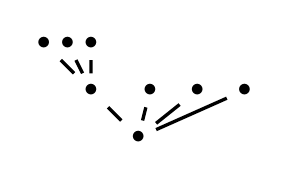
\begin{tikzpicture}[very thick, scale=0.3]
  \node (h1) at (4,0){$\bullet$};
  \node (h2) at (2,2){$\bullet$};
  \node (h3) at (0,4){$\bullet$};
  \node (h4) at (1,4){$\bullet$};
  \node (h5) at (2,4){$\bullet$};
  \node (h6) at (4.5,2){$\bullet$};
  \node (h7) at (6.5,2){$\bullet$};
  \node (h8) at (8.5,2){$\bullet$};
    \draw (h1) -- (h2) ;
    \draw (h2) -- (h3) ;
    \draw (h2) -- (h4) ;
    \draw (h2) -- (h5) ;
    \draw (h1) -- (h6) ;
    \draw (h1) -- (h7) ;
    \draw (h1) -- (h8);
 \end{tikzpicture}

  \caption{The hydra corresponding to the ordinal $\omega^3+3$}
  \label{fig:start}
\end{figure}




\section{A variant of the Wainer hierarchy (functions \texorpdfstring{$F_\alpha$}{F\_alpha})}
\label{sect:wainer}

\index{maths}{Rapidly growing functions!Wainer Hierarchy}

Ketonen and Solovay introduce in~\cite{KS81} a ``trivial'' variant of the Wainer hierarchy~\cite{BW85, Wainer1970} of fast growing functions, indexed by ordinals below $\epsilon_0$.
The functions $F_\alpha$ are defined by the following equations.

\label{F_equations}
\begin{itemize}
\item $F_0(i)=i+1$
\item $F_{\beta+1}(i)= (F_\beta)^{(i+1)}(i)$, where $f^{(i)}$ is the $i$-th iterate of $f$.
\item $F_\alpha(i) = F_{\canonseq{\alpha}{i}} (i)$ if $\alpha$ is a limit ordinal.
\end{itemize}

\begin{remark}
The difference with the ``classic'' Wainer hierarchy 
$f_\alpha\;(\alpha<\epsilon_0)$ lies in the second equation:
$f_{\beta+1}(i) = (f_\beta)^{(i)}(i)$ and not
$f_{\beta+1}(i) = (f_\beta)^{(i+1)}(i)$.

A module about 
the classic Wainer hierarchy is in preparation.

Note also that \cite{KS81} defines also $F_{\epsilon_0}$ (by the third equation). Since $\epsilon_0$ is not representable in type \texttt{E0}, our implementation in \coq{} does not take $F_{\epsilon_0}$ into account.

\end{remark}

A first attempt is to write a definition of $F_\alpha$ by equations, in the same way as for $H_\alpha$ (the functional \texttt{iterate} has already been used in Sect.\vref{Functions:iterate}).



\index{hydras}{Library Prelude!iterate}

\input{movies/snippets/Iterates/iterateDef}


\emph{From\href{../theories/html/hydras.Epsilon0.F_alpha.html}{Epsilon0.F\_alpha}~}.

\index{coq}{Plug-ins!Equations}

 \input{movies/snippets/F_alpha/FailDemo}
 


We presume that this error comes from the recursive call of \texttt{F\_} inside
an application of \texttt{iterate}. The workaround we propose is to define first 
the iteration of \texttt{F\_}  as an helper $F^*$, then to define the function $F$ as a ``iterating $F^*$ once''.

\texttt{Equations} accepts the following definition, relying on  lexicographic ordering on pairs $(\alpha,n)$.


\label{sect:F-equations}

\index{coq}{Plug-ins!Equations}
\label{Functions:F-alpha}
\index{maths}{Rapidly growing functions}
\index{hydras}{Library Epsilon0!Functions!F\_@F\_ (Wainer hierarchy)}
  
\input{movies/snippets/F_alpha/goodDefa}
\input{movies/snippets/F_alpha/goodDefb}


It is quite easy to prove that our functional \texttt{F\_} satisfies the equations on page~\pageref{sect:F-equations}.
\index{hydras}{Library Prelude!iterate}

\input{movies/snippets/F_alpha/FEquations}


As for the Hardy functions, we can use these equalities as rewrite rules for
``computing'' some values of $F_\alpha(i)$, for small values of $\alpha$.

\input{movies/snippets/F_alpha/FirstValues}

Like in Sect~\ref{sect:H-alpha-prop}, we prove by induction the following properties (see~\cite{KS81}). 

\input{movies/snippets/F_alpha/FalphaThms}


As a corollary, we prove that, if $\beta<\alpha$, then
$F_\alpha$ dominates $F_\beta$ (p. 284 of~\cite{KS81}).

\input{movies/snippets/F_alpha/FDomContext}
\input{movies/snippets/F_alpha/FDom}


\index{hydras}{Exercises}

\begin{exercise}
Prove the following property:

\begin{Coqsrc}
Lemma LF3 : dominates_from  2 (F_ 3) (fun  n => iterate exp2 n n).
\end{Coqsrc}

\emph{You may start this exercise with the file
\href{https://github.com/coq-community/hydra-battles/tree/master/exercises/ordinals/F_3.v}{exercises/ordinals/F\_3.v}.}
\end{exercise}

\index{hydras}{Exercises}

\begin{exercise}
Prove that, for any $\alpha\geq 3$ and $n\geq 2$,
$F_\alpha(1+n)\geq 2^{F_\alpha(n)}$.



\emph{You may start this exercise with the file
    \href{https://github.com/coq-community/hydra-battles/tree/master/exercises/ordinals/F_3.v}{exercises/ordinals/F\_3.v}.}
\end{exercise}


%ici
\index{hydras}{Exercises}

\begin{exercise}
It is tempting to prove a simple property of monotony 
of the function \texttt{F\_}.

\begin{quote}
   Let $\alpha\leq\beta<\epsilon_0$. For any $n\geq 2$,
$F_\alpha(n)\leq F_\beta(n)$. 
\end{quote}
Prove or disprove this statement.

\emph{You may start this exercise with the file
    \href{https://github.com/coq-community/hydra-battles/tree/master/exercises/ordinals/is_F_monotonous.v}{exercises/ordinals/is\_F\_monotonous.v}.}
\end{exercise}

\index{hydras}{Exercises}
\begin{exercise}



Prove that for any $n\geq 2$, $\textrm{Ack}\,\,n\,n\leq  F_\omega(n)$, where \textrm{Ack} is the Ackermann function. Next, prove that $F_\alpha$ is not primitive recursive, for any $\alpha\geq\omega$  (please see Sect.~\vref{sect:ack-not-PR}).
On the other hand, please show that for any natural number $n$, the function $F_n$ is primitive recursive.
Thus $F_\alpha$ is primitive recursive if and only if $\alpha$ is finite.

\emph{You may start this exercise with the file
    \href{https://github.com/coq-community/hydra-battles/tree/master/exercises/ordinals/F_omega.v}{exercises/ordinals/F\_Omega.v}.
Properties of the Ackermann function are studied in
    \href{https://github.com/coq-community/hydra-battles/tree/master/theories/ordinals/MoreAck/Ack.v}{theories/ordinals/MoreAck/Ack.v} and
    \href{https://github.com/coq-community/hydra-battles/tree/master/theories/ordinals/MoreAck/AckNotPR.v}{theories/ordinals/MoreAck/AckNotPR.v}
.}
\end{exercise} 

\paragraph*{\gaiasign} Library~\href{../theories/html/gaia_hydras.GF_alpha.html}{gaia\_hydras.GF\_alpha}  defines the functions $F_\alpha$ for \gaia's world.
\index{gaiabridge}{Rapidly growing functions}

\section{More about rapidly growing functions}

In Sect.~\vref{sect:battle-length-notPR}, we prove that the length of hydra-battles (for a given hydra, according to the initial replication factor) is not primitive recursive in general. 
This proof uses properties of the Ackermann function, and the $H'_\alpha$, $F_\alpha$, $L_\alpha$ families of functions.


